\section{Code}

\subsection{Korrelation}
\lstinputlisting{fig/code/hainich-correlation.r}

\subsubsection{Korrelation der Temperatur}
\lstinputlisting{fig/code/hainich-correlation-temp-resp.r}

\subsection{Variablenselektion}
\lstinputlisting{fig/code/hainich-variablenselektion.r}

\subsection{Simulation}
\subsubsection{Monte-Carlo}
\lstinputlisting{fig/code/hainich-f-simul-monte.r}
\subsubsection{Kreuzvalidierung}
\lstinputlisting{fig/code/hainich-f-simul-crossval.r}

\newpage
\FloatBarrier
\section{Appendix}

\begin{figure}[h!]
	\centering
	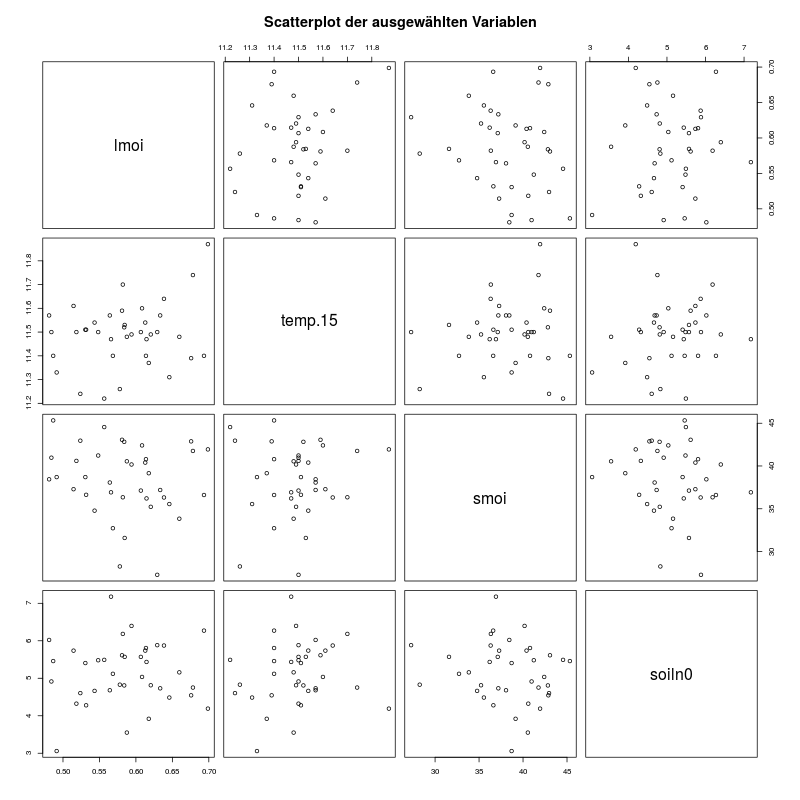
\includegraphics[width=0.9\textwidth]{fig/model/scatterplot-pearson-normalverteilt.png}
	\caption{Scatterplot zur Betrachtung der Korrelation der ausgewählten Variablen}
	\label{fig:scatter-top4}
\end{figure}

